\documentclass{article}
\usepackage{graphicx}
\graphicspath{ {/asay/Desktop/images/} }
\usepackage{color}
\usepackage{xcolor}
\usepackage{xepersian}


\title{پاسخ تمرین تئوری ۱ درس هوش مصنوعی  }
\author{امیر حسین عاصم یوسفی \\ ۹۶۱۱۰۳۲۳}
\settextfont{B Nazanin}


\begin{document}
	\maketitle
	
	\section*{سوال ۱ }
	جدول به صورت زیر می باشد  : 
	\begin{center}
		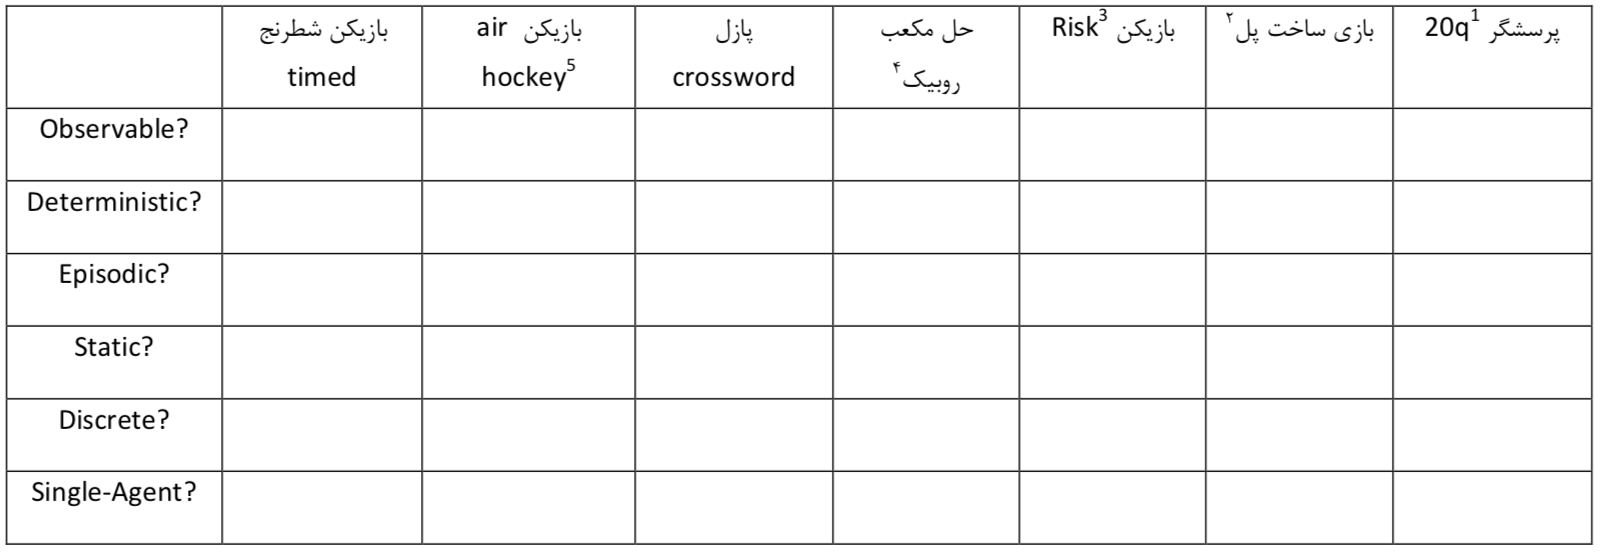
\includegraphics[width=1\textwidth]{table}
	\end{center}
	
	\hrule
	\section*{سوال ۲ }
	ابتدا گراف داده شده را به شکل زیر بازنویسی می کنیم  : 
	\begin{center}
	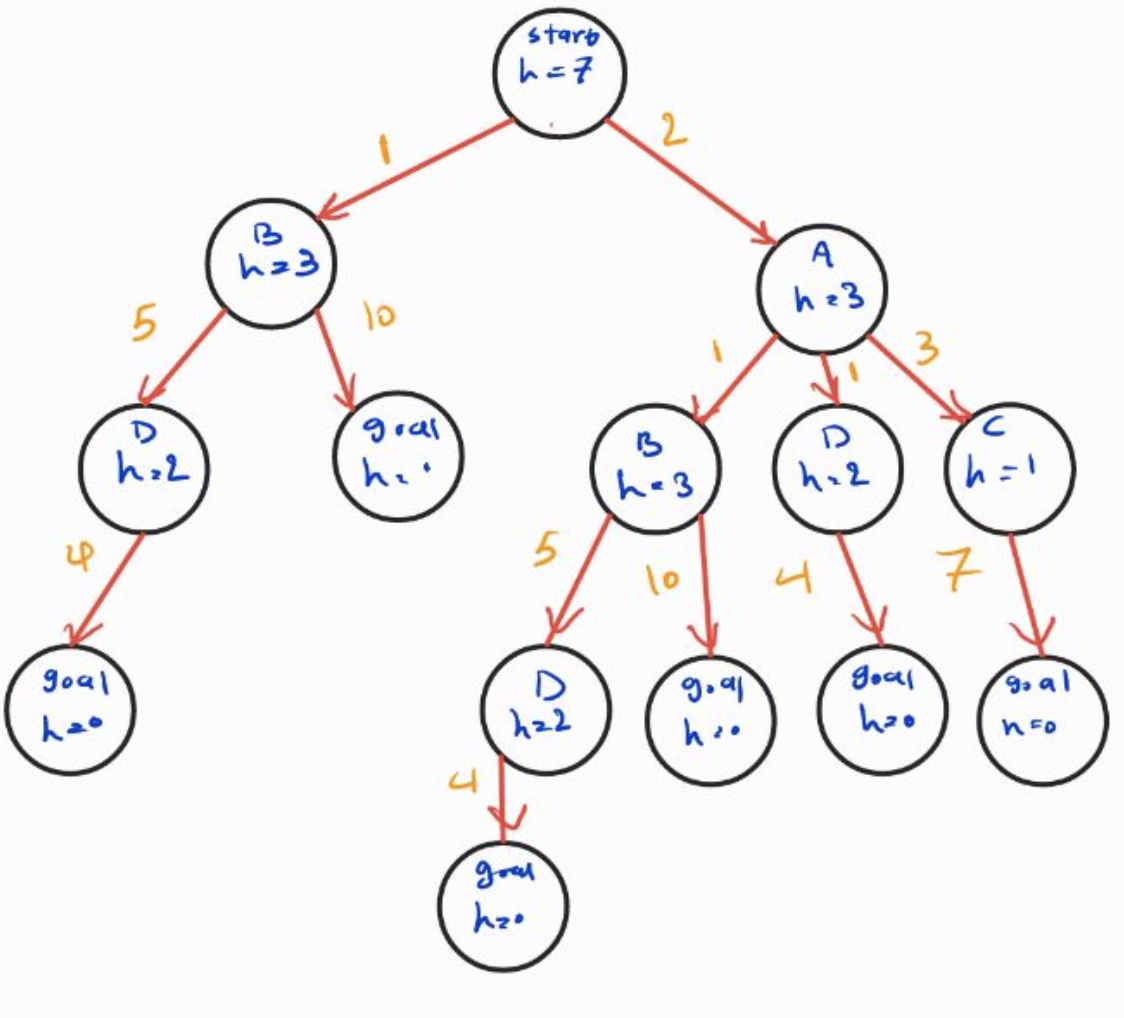
\includegraphics[width=0.5\textwidth]{q2p1}
\end{center}
\newpage
\subsection*{\textcolor{red}{\lr{BFS}}}
با توجه به این که این روش یک روش جستجو 
\lr{Uninformed}
 می باشد بنابراین نیازی به  مقدار تابع 
 \lr{h}
  و طول یال ها برای انجام این الگوریتم نیست و فقط باید این را درنظر داشته باشیم که باید ترتیب الفبایی را رعایت کنیم   . \\
برای اجرای این الگوریتم دو صف به نام های 
\lr{Visited}
و 
\lr{Exapnded}
در نظر می گیریم  : 
\subsubsection*{مرحله ۱ }
\begin{center}
	\begin{enumerate}
		\item  \lr{Visited  : S }
		\item  \lr{Expanded : empty}
		\end{enumerate}
\end{center}
\subsubsection*{مرحله ۲}
\begin{center}
	\begin{enumerate}
		\item \lr{Visited  : A  , B}
		\item \lr{Expanded : S}
	\end{enumerate}
\end{center}
\subsubsection*{مرحله ۳ }
\begin{center}
	\begin{enumerate}
		\item  \lr{Visited  : ‌‌‌ B  , C , D}
		\item  \lr{Expanded : S , A }
	\end{enumerate}
\end{center}
\subsubsection*{مرحله ۴ }
\begin{center}
	\begin{enumerate}
		\item  \lr{Visited  : ‌‌‌  C , D , Goal  }
		\item  \lr{Expanded : S , A , B }
	\end{enumerate}
\end{center}
\subsubsection*{مرحله ۵ }
\begin{center}
	\begin{enumerate}
		\item  \lr{Visited  : ‌‌‌ D  , Goal }
		\item  \lr{Expanded : S , A , B , C }
	\end{enumerate}
\end{center}
\subsubsection*{مرحله ۶ }
\begin{center}
	\begin{enumerate}
		\item  \lr{Visited  : ‌‌‌ Goal }
		\item  \lr{Expanded : S , A , B , C , D }
	\end{enumerate}
\end{center}
\subsubsection*{مرحله ۷ }
\begin{center}
	\begin{enumerate}
		\item  \lr{Visited  : ‌‌‌ empty}
		\item  \lr{Expanded : S , A , B , C , D ,Goal }
	\end{enumerate}
\end{center}
\newpage
\subsection*{\textcolor{red}{\lr{DFS}}}
در این الگوریتم در عمق پایین می رویم تا به گره هدف برسیم و تنها باید ترتیب الفبایی را رعایت کنیم  : 
\subsubsection*{مرحله ۱ }
\begin{center}
	\begin{enumerate}
		\item  \lr{Visited  : ‌‌‌ S }
		\item  \lr{Expanded : empty }
	\end{enumerate}
\end{center}
\subsubsection*{مرحله ۲ }
\begin{center}
	\begin{enumerate}
		\item  \lr{Visited  : ‌‌‌ A , B  }
		\item  \lr{Expanded : S }
	\end{enumerate}
\end{center}
\subsubsection*{مرحله ۳ }
\begin{center}
	\begin{enumerate}
		\item  \lr{Visited  : ‌‌‌ C }
		\item  \lr{Expanded : S , A}
	\end{enumerate}
\end{center}
\subsubsection*{مرحله ۴ }
\begin{center}
	\begin{enumerate}
		\item  \lr{Visited  : ‌‌‌ Goal }
		\item  \lr{Expanded : S , A , C  }
	\end{enumerate}
\end{center}
\subsubsection*{مرحله ۵ }
\begin{center}
	\begin{enumerate}
		\item  \lr{Visited  : ‌‌‌empty }
		\item  \lr{Expanded : S , A , C , Goal  }
	\end{enumerate}
\end{center}
\section*{\textcolor{red}{\lr{UCS}}}
در این الگوریتم گره ای را 
\lr{Expand}
می کنیم 
\lr{Path Cost}
کمتری دارد  : 
\subsubsection*{مرحله ۱ }
\begin{center}
\lr{Iteration 1 : [S -> B  , 1] , [S -> A , 2]}
\end{center}
\subsubsection*{مرحله ۲ }
\begin{center}
	\lr{Iteration 2 : [S -> A -> B , 3] , [S -> A -> D , 3] , [S -> A -> C , 5] , [S -> B -> D , 6] , [S -> B -> G , 11]}
\end{center}
\subsubsection*{مرحله ۳ }
\begin{center}
	\lr{Iteration 3 : [S -> A -> B -> G , 13] , [S -> A ->D -> G , 7], [S -> A -> C -> G-> , 12] , [A -> B -> D -> G  , 12], 
	[S -> B -> G - , 11]}
\end{center}
در هر مرحله چون همواره یک لیست مرتب شده داریم بنابراین 
\lr{[S -> A -> D -> G , 7]}
در اولویت قرار می گیرد بنابراین در مرحله بعدی جواب بهینه که مسیر گفته شده را طی می کند از صف بیرون آمده و جستجو تمام می شود . 
\subsection*{\textcolor{red}{\lr{ID DFS}}}
برای این الگوریتم باید هر بار با یک
\lr{Limit}
جدید  به جستجو به صورت 
\lr{DFS}
ادامه دهیم  . 
که  به صورت زیر است  : 
	\begin{center}
	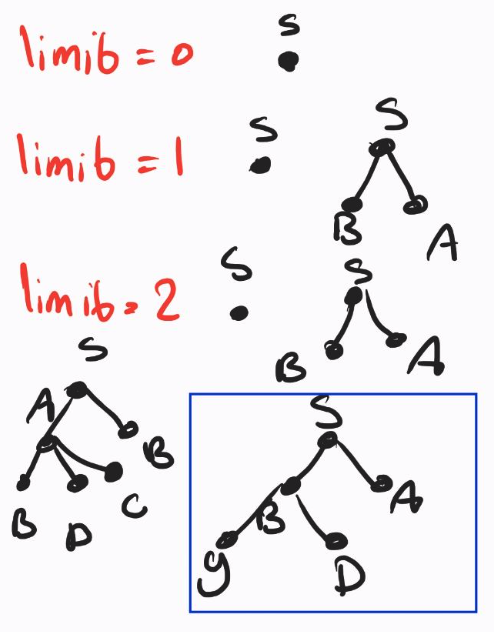
\includegraphics[width=0.5\textwidth]{iddfs}
\end{center}
\subsection*{\textcolor{red}{\lr{A *}}}
برای این الگوریتم هربار باید مقدار 
\lr{F =g + h}
را برای هر گره حساب کنیم و هر بار گره ای را 
\lr{Expand}
می کنیم که کمترین 
\lr{F}
را دارد  . 
\\
در این الگوریتم اگر به یک حالت تکراری با مقدار 
\lr{F}
بهتر رسیدیم که هنوز 
\lr{Expand}
نشده است مقدار بهتر را جایگزین می کنیم  . 
	\begin{center}
	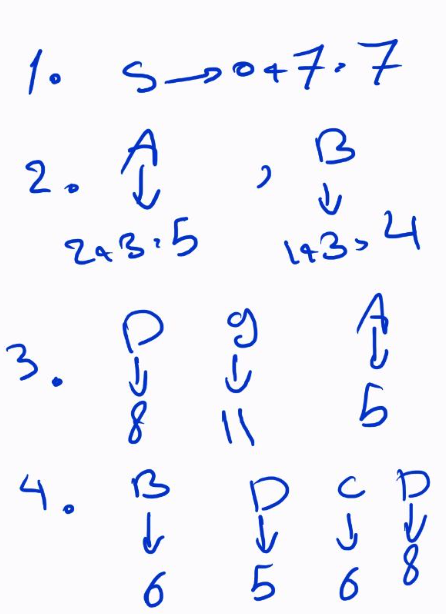
\includegraphics[width=0.4\textwidth]{q2p2}
\end{center}
در این مرحله چون یک بار گره 
\lr{B}
را 
\lr{Expand}
کرده ایم آن را از صف حذف می کنیم . \\
همچنین در این حالت همان طور که می توان دید به گره 
\lr{D}
با دو مقدار مختلف رسیدیم که یکی از طریق گره 
\lr{A}
با مقدار 
\lr{F = 5}
و دیگری از مسیر گره 
\lr{B}
با مقدار 
\lr{F = 8}
که در این جا بهترین گره رو نگه می داریم و مراحل به صورت زیر می شود  : 
\begin{center}
	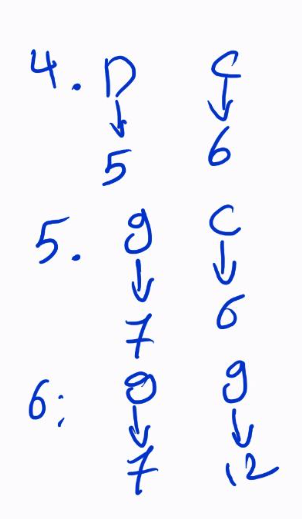
\includegraphics[width=0.4\textwidth]{q2p3}
\end{center}
و در مرحله ۶ ام با دو مقدار متفاوت 
\lr{F}
به گره هدف رسیدیم که در این جا بهترین گره را نگه میداریم بنابراین 
\lr{Exapnsion Order }
به صورت زیر می باشد : 
\begin{center}
	\begin{enumerate}
		\item \lr{S , F = 7}
		\item \lr{B  , F = 4}
		\item \lr{A , F = 5}
		\item \lr{D  , F = 5}
		\item \lr{C , F = 6}
		\item \lr{Goal , F = 7}
		\end{enumerate}
\end{center}
\hrule
\newpage
\section*{سوال ۳}
ابتدا گراف داده شده را به صورت زیر بازنویسی می کنیم  : 
	\begin{center}
	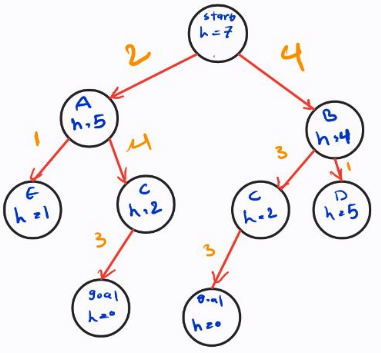
\includegraphics[width=0.4\textwidth]{q3p1}
\end{center}


\subsection*{\textcolor{red}{\lr{Best - First Search}}}
در این روش تنها به مقدار 
\lr{Heuristic}
توجه می کنیم و همواره گره ای را 
\lr{Expand}
می کنیم که کمترین 
\lr{Heuristic}
را دارد . که به صورت زیر می باشد : 
\begin{center}
	\begin{enumerate}
		\item \lr{S ,  h = 7}
		\item \lr{B , h= 4}
		\item \lr{C , h = 2}
		\item \lr{G = 0}
	\end{enumerate}
\end{center}
بنابراین مسیری که این الگوریتم پیدا می کند به صورت 
\lr{S -> B -> C -> G}
می باشد  . 
\subsection*{\textcolor{red}{\lr{A *}}}
برای این الگوریتم 
\lr{Expansion Order }
به صورت زیر می باشد : 
\begin{center}
	\begin{enumerate}
	 \item \lr{S , F = 7}
	 \item \lr{A , F = 7}
	 \item \lr{E , F = 4}
	 \item \lr{B  , F = 8}
	 \item \lr{C   , F = 8}
	 \item \lr{Goal , F = 9}
	\end{enumerate}
\end{center}
بنابراین مسیری که این الگوریتم طی میکند به صورت 
\lr{S -> A -> C -> G}
می باشد 
\subsection*{\textcolor{red}{\lr{IDA *}}}
در این الگوریتم هر بار یک 
\lr{Limit }
جدید برای مقدار 
\lr{F}
مشخص می کنیم اگر در آن مرحله به گره هدف رسیدیم که کار تمام است ولی اگر این اتفاق نیافتاد از بین آن هایی که از محدودیت ما بیشتر هستند کمترین را برای 
\lr{Limit}
مرحله بعد انتخاب می کنیم بنابراین داریم  : 
\subsubsection*{\lr{Limit = 7}}
\begin{center}
	\begin{enumerate}
		\item \lr{S , F = 7}
		\item \lr{A , F = 7}
		\item \lr{E , F = 4}
	\end{enumerate}
\end{center}
در این مرحله به گره هدف نرسیدیم پس این بار 
\lr{Limit   = 8}
\subsubsection*{\lr{Limit = 8 }}
\begin{center}
	\begin{enumerate}
		\item \lr{S , F = 7}
		\item \lr{A , F = 7}
		\item \lr{E , F = 4}
		\item \lr{C  , F = 8}
	\end{enumerate}
\end{center}
در این مرحله فرزند 
\lr{C}
که گره هدف است مقدار 
\lr{F = 9}
را دارد بنابراین الگوریم با توجه به محدودیت آن را از صف بیرون نمی آورد پس این بار با 
\lr{Limit = 9}
انجام می دهیم  .
\subsubsection*{\lr{Limit = 9 }}
 \begin{center}
 	\begin{enumerate}
 		\item \lr{S , F = 7}
 		\item \lr{A , F = 7}
 		\item \lr{E , F = 4}
 		\item \lr{C  , F = 8}
 		\item \lr{G , F = 9}
 	\end{enumerate}
 \end{center}
بنابراین مسیری که این الگوریتم طی میکند به صورت 
\lr{S -> A -> C -> G}
می باشد 
\subsubsection*{\textcolor{red}{\lr{ID DFS}}}
این الگوریتم به صورت زیر می باشد : 
	\begin{center}
	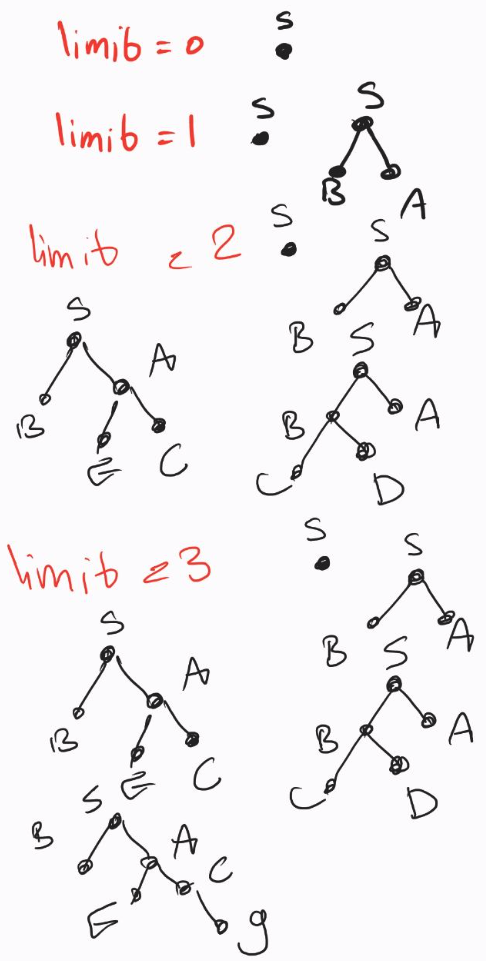
\includegraphics[width=0.25\textwidth]{q3p2}
\end{center}

\section*{سوال ۴}
\subsection*{\textcolor{red}{الف}}
\begin{center}
	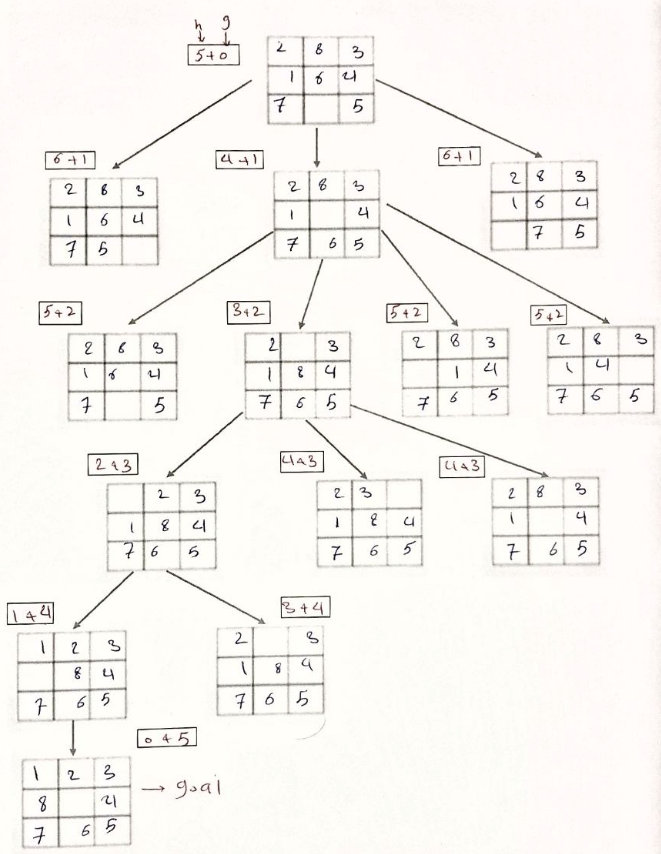
\includegraphics[width=0.5\textwidth]{q4p1}
\end{center}
\subsection*{\textcolor{red}{ب}}
خیر ، زیرا ممکن است در 
\lr{Local Maxima}
به دام بیافتیم و هیچ گاه به بلندترین قله نرسیم 
\\
دلیل دیگر این است که ممکن است فلات داشته باشیم یعنی مقدار 
\lr{Heuristic}
تغییری نکند  . 
\hrule
\section*{سوال ۵ }
با اجرای الگوریتم گفته شده به نتیجه زیر می رسیم : 
\begin{center}
	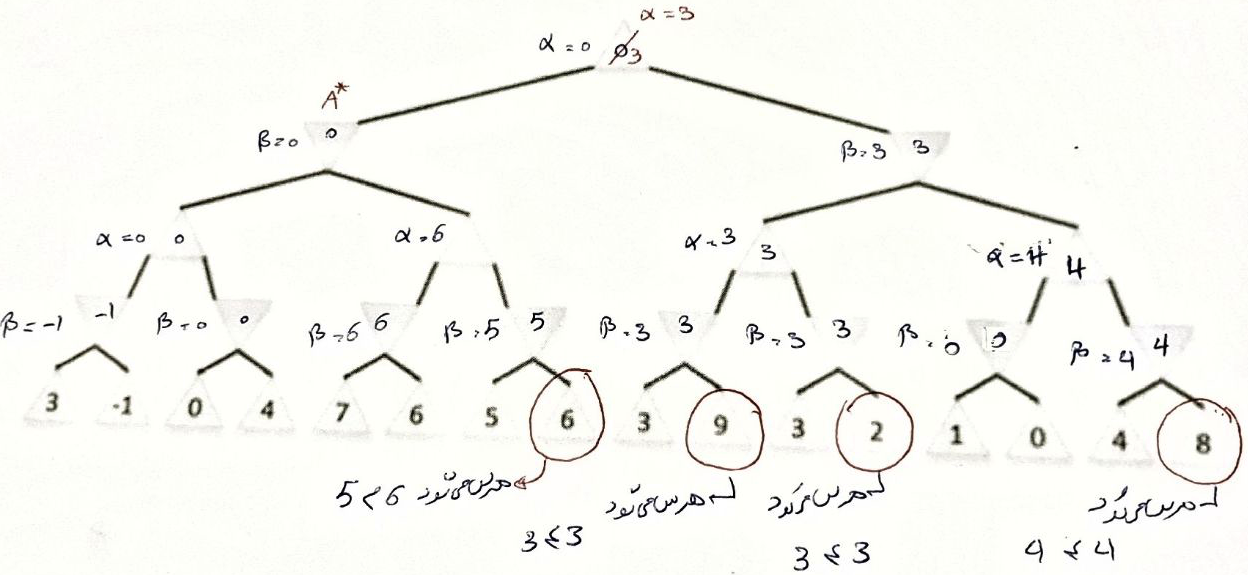
\includegraphics[width=1.1\textwidth]{q5p1}
\end{center}
\section*{سوال ۶}
\subsection*{\textcolor{red}{الف}}
با توجه به فرضی که در قسمت ب گفته شده اگر این مسئله را به روش ارضا محدودیت حل کنیم نیازی به 
\lr{Backtrack}
نداریم زیرا در هر مرحله با توجه به این ترتیب الفبایی هم درمقدار دادن به کشورها و هم در رنگ ها وجود همواره در اولین مرحله به افغانستان (ترتیب الفبایی در کشورها) رنگ آبی (ترتیب الفبایی در رنگ ها) و بنابراین مقدار دهی به ترتیب زیر می باشد  : 
\begin{center}
	\begin{enumerate}
		\item \lr{Afghanistan}
		\item \lr{Iran}
		\item \lr{Iraq}
		\item \lr{Turkey}
		\item \lr{Turkmenistan}
		\item \lr{Saudi Arabia}
	\end{enumerate}
\end{center}
اما اگر فرض موجود در قسمت ب وجود نداشت می توانستیم ابتدا به افغانستان  و بعدد به ترکمنستان و بعد ترکیه مقدار دهیم آنگاه هیچ مقداری برای ایران باقی نمی ماند و در ابن صورت مجبور به 
\lr{Backtrack}
بودیم  . 
\subsection*{\textcolor{red}{ب}}
برای این قسمت ابتدا گراف محدودیت را رسم می کنیم که به صورت زیر می باشد  : 
\begin{center}
	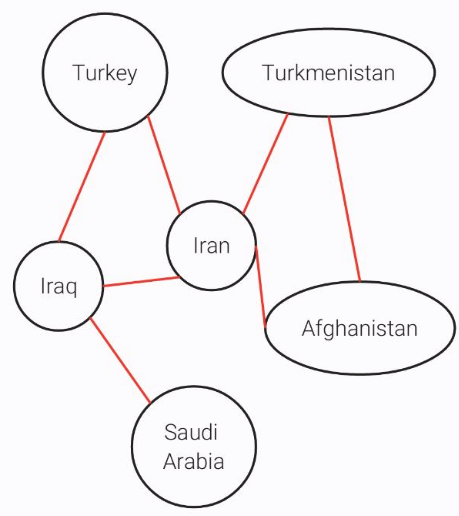
\includegraphics[width=0.4\textwidth]{q6p1}
\end{center}
حال با توجه به این گراف محدودیت روش های گفته شده را پیاده سازی می کنیم  . 
\subsubsection*{\textcolor{red}{\lr{FC}}}
\begin{center}
	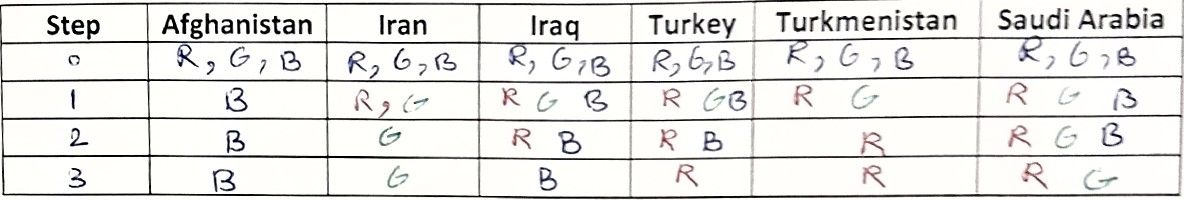
\includegraphics[width=1\textwidth]{fc}
\end{center}
\subsubsection*{\textcolor{red}{\lr{PL}}}
در این الگوریتم در هر مرحله فقط تاثیر دو متغیر را بر یکدیگر بررسی می کنیم  . \\
همچنین در این الگوریتم همواره بعد از مقداردهی 
\lr{Forward Checking}
انجام می دهیم  . 
در مرحله اول به افغانستان مقدار می دهیم و داریم  : 
\begin{center}
	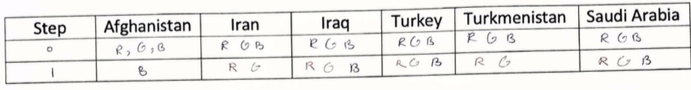
\includegraphics[width=1\textwidth]{q6p2}
\end{center}
در همین   مرحله تاثیر دو متغیری که مقدار نگرفته اند (ایران و عراق) را برهم بررسی می کنیم و داریم  : 
\begin{center}
	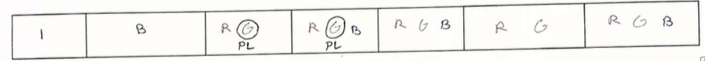
\includegraphics[width=1\textwidth]{q6p3}
\end{center}
در مرحله دوم  با توجه به تصویر بالا رنگ قرمز را به ایران می دهیم و حال با استفاده از 
\lr{Forward Checking}
داریم : 
\begin{center}
	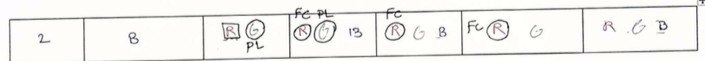
\includegraphics[width=1\textwidth]{q6p4}
\end{center}
که در نهایت برای مرحله دو به جدول زیر می رسیم   : 
\begin{center}
	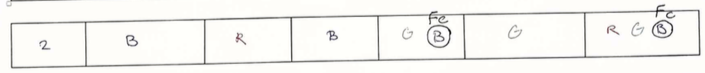
\includegraphics[width=1\textwidth]{q6p5}
\end{center}
در مرحله سوم حال به عراق تنها مقدار باقی مانده برای آن (آبی) را اختصاص می دهیم و با استفاده از 
\lr{Forward Checking}
داریم  : 
\begin{center}
	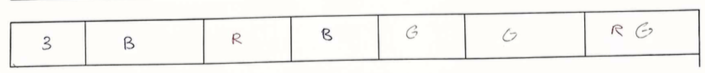
\includegraphics[width=1\textwidth]{q6p6}
\end{center}
\subsubsection*{\textcolor{red}{\lr{FL}}}
در این الگوریتم تاثیر هر دو متغیری که مقدار نگرفته اند را نسبت به هم بررسی می کنیم  . و در هر مرحله بعد از این که از دامنه متغیرها با استفاده از 
\lr{Fully  Look Ahead}
مقادیر غیر مجاز را حذف کردیم  و بعد از مقدار دادن به یک متغیر الگوریتم 
\lr{Forward Checking}
  را اعمال کنیم . که با انجام دادن این مراحل به جدول زیر می رسیم  : 
  
\begin{center}
	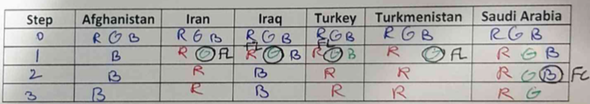
\includegraphics[width=1\textwidth]{q6p7}
\end{center}

\end{document}
